% Options for packages loaded elsewhere
\PassOptionsToPackage{unicode}{hyperref}
\PassOptionsToPackage{hyphens}{url}
\PassOptionsToPackage{dvipsnames,svgnames,x11names}{xcolor}
%
\documentclass[
  letterpaper,
  DIV=11,
  numbers=noendperiod]{scrreprt}

\usepackage{amsmath,amssymb}
\usepackage{lmodern}
\usepackage{iftex}
\ifPDFTeX
  \usepackage[T1]{fontenc}
  \usepackage[utf8]{inputenc}
  \usepackage{textcomp} % provide euro and other symbols
\else % if luatex or xetex
  \usepackage{unicode-math}
  \defaultfontfeatures{Scale=MatchLowercase}
  \defaultfontfeatures[\rmfamily]{Ligatures=TeX,Scale=1}
\fi
% Use upquote if available, for straight quotes in verbatim environments
\IfFileExists{upquote.sty}{\usepackage{upquote}}{}
\IfFileExists{microtype.sty}{% use microtype if available
  \usepackage[]{microtype}
  \UseMicrotypeSet[protrusion]{basicmath} % disable protrusion for tt fonts
}{}
\makeatletter
\@ifundefined{KOMAClassName}{% if non-KOMA class
  \IfFileExists{parskip.sty}{%
    \usepackage{parskip}
  }{% else
    \setlength{\parindent}{0pt}
    \setlength{\parskip}{6pt plus 2pt minus 1pt}}
}{% if KOMA class
  \KOMAoptions{parskip=half}}
\makeatother
\usepackage{xcolor}
\setlength{\emergencystretch}{3em} % prevent overfull lines
\setcounter{secnumdepth}{5}
% Make \paragraph and \subparagraph free-standing
\ifx\paragraph\undefined\else
  \let\oldparagraph\paragraph
  \renewcommand{\paragraph}[1]{\oldparagraph{#1}\mbox{}}
\fi
\ifx\subparagraph\undefined\else
  \let\oldsubparagraph\subparagraph
  \renewcommand{\subparagraph}[1]{\oldsubparagraph{#1}\mbox{}}
\fi

\usepackage{color}
\usepackage{fancyvrb}
\newcommand{\VerbBar}{|}
\newcommand{\VERB}{\Verb[commandchars=\\\{\}]}
\DefineVerbatimEnvironment{Highlighting}{Verbatim}{commandchars=\\\{\}}
% Add ',fontsize=\small' for more characters per line
\usepackage{framed}
\definecolor{shadecolor}{RGB}{241,243,245}
\newenvironment{Shaded}{\begin{snugshade}}{\end{snugshade}}
\newcommand{\AlertTok}[1]{\textcolor[rgb]{0.68,0.00,0.00}{#1}}
\newcommand{\AnnotationTok}[1]{\textcolor[rgb]{0.37,0.37,0.37}{#1}}
\newcommand{\AttributeTok}[1]{\textcolor[rgb]{0.40,0.45,0.13}{#1}}
\newcommand{\BaseNTok}[1]{\textcolor[rgb]{0.68,0.00,0.00}{#1}}
\newcommand{\BuiltInTok}[1]{\textcolor[rgb]{0.00,0.23,0.31}{#1}}
\newcommand{\CharTok}[1]{\textcolor[rgb]{0.13,0.47,0.30}{#1}}
\newcommand{\CommentTok}[1]{\textcolor[rgb]{0.37,0.37,0.37}{#1}}
\newcommand{\CommentVarTok}[1]{\textcolor[rgb]{0.37,0.37,0.37}{\textit{#1}}}
\newcommand{\ConstantTok}[1]{\textcolor[rgb]{0.56,0.35,0.01}{#1}}
\newcommand{\ControlFlowTok}[1]{\textcolor[rgb]{0.00,0.23,0.31}{#1}}
\newcommand{\DataTypeTok}[1]{\textcolor[rgb]{0.68,0.00,0.00}{#1}}
\newcommand{\DecValTok}[1]{\textcolor[rgb]{0.68,0.00,0.00}{#1}}
\newcommand{\DocumentationTok}[1]{\textcolor[rgb]{0.37,0.37,0.37}{\textit{#1}}}
\newcommand{\ErrorTok}[1]{\textcolor[rgb]{0.68,0.00,0.00}{#1}}
\newcommand{\ExtensionTok}[1]{\textcolor[rgb]{0.00,0.23,0.31}{#1}}
\newcommand{\FloatTok}[1]{\textcolor[rgb]{0.68,0.00,0.00}{#1}}
\newcommand{\FunctionTok}[1]{\textcolor[rgb]{0.28,0.35,0.67}{#1}}
\newcommand{\ImportTok}[1]{\textcolor[rgb]{0.00,0.46,0.62}{#1}}
\newcommand{\InformationTok}[1]{\textcolor[rgb]{0.37,0.37,0.37}{#1}}
\newcommand{\KeywordTok}[1]{\textcolor[rgb]{0.00,0.23,0.31}{#1}}
\newcommand{\NormalTok}[1]{\textcolor[rgb]{0.00,0.23,0.31}{#1}}
\newcommand{\OperatorTok}[1]{\textcolor[rgb]{0.37,0.37,0.37}{#1}}
\newcommand{\OtherTok}[1]{\textcolor[rgb]{0.00,0.23,0.31}{#1}}
\newcommand{\PreprocessorTok}[1]{\textcolor[rgb]{0.68,0.00,0.00}{#1}}
\newcommand{\RegionMarkerTok}[1]{\textcolor[rgb]{0.00,0.23,0.31}{#1}}
\newcommand{\SpecialCharTok}[1]{\textcolor[rgb]{0.37,0.37,0.37}{#1}}
\newcommand{\SpecialStringTok}[1]{\textcolor[rgb]{0.13,0.47,0.30}{#1}}
\newcommand{\StringTok}[1]{\textcolor[rgb]{0.13,0.47,0.30}{#1}}
\newcommand{\VariableTok}[1]{\textcolor[rgb]{0.07,0.07,0.07}{#1}}
\newcommand{\VerbatimStringTok}[1]{\textcolor[rgb]{0.13,0.47,0.30}{#1}}
\newcommand{\WarningTok}[1]{\textcolor[rgb]{0.37,0.37,0.37}{\textit{#1}}}

\providecommand{\tightlist}{%
  \setlength{\itemsep}{0pt}\setlength{\parskip}{0pt}}\usepackage{longtable,booktabs,array}
\usepackage{calc} % for calculating minipage widths
% Correct order of tables after \paragraph or \subparagraph
\usepackage{etoolbox}
\makeatletter
\patchcmd\longtable{\par}{\if@noskipsec\mbox{}\fi\par}{}{}
\makeatother
% Allow footnotes in longtable head/foot
\IfFileExists{footnotehyper.sty}{\usepackage{footnotehyper}}{\usepackage{footnote}}
\makesavenoteenv{longtable}
\usepackage{graphicx}
\makeatletter
\def\maxwidth{\ifdim\Gin@nat@width>\linewidth\linewidth\else\Gin@nat@width\fi}
\def\maxheight{\ifdim\Gin@nat@height>\textheight\textheight\else\Gin@nat@height\fi}
\makeatother
% Scale images if necessary, so that they will not overflow the page
% margins by default, and it is still possible to overwrite the defaults
% using explicit options in \includegraphics[width, height, ...]{}
\setkeys{Gin}{width=\maxwidth,height=\maxheight,keepaspectratio}
% Set default figure placement to htbp
\makeatletter
\def\fps@figure{htbp}
\makeatother

\KOMAoption{captions}{tableheading}
\makeatletter
\makeatother
\makeatletter
\@ifpackageloaded{bookmark}{}{\usepackage{bookmark}}
\makeatother
\makeatletter
\@ifpackageloaded{caption}{}{\usepackage{caption}}
\AtBeginDocument{%
\ifdefined\contentsname
  \renewcommand*\contentsname{Table of contents}
\else
  \newcommand\contentsname{Table of contents}
\fi
\ifdefined\listfigurename
  \renewcommand*\listfigurename{List of Figures}
\else
  \newcommand\listfigurename{List of Figures}
\fi
\ifdefined\listtablename
  \renewcommand*\listtablename{List of Tables}
\else
  \newcommand\listtablename{List of Tables}
\fi
\ifdefined\figurename
  \renewcommand*\figurename{Figure}
\else
  \newcommand\figurename{Figure}
\fi
\ifdefined\tablename
  \renewcommand*\tablename{Table}
\else
  \newcommand\tablename{Table}
\fi
}
\@ifpackageloaded{float}{}{\usepackage{float}}
\floatstyle{ruled}
\@ifundefined{c@chapter}{\newfloat{codelisting}{h}{lop}}{\newfloat{codelisting}{h}{lop}[chapter]}
\floatname{codelisting}{Listing}
\newcommand*\listoflistings{\listof{codelisting}{List of Listings}}
\makeatother
\makeatletter
\@ifpackageloaded{caption}{}{\usepackage{caption}}
\@ifpackageloaded{subcaption}{}{\usepackage{subcaption}}
\makeatother
\makeatletter
\@ifpackageloaded{tcolorbox}{}{\usepackage[many]{tcolorbox}}
\makeatother
\makeatletter
\@ifundefined{shadecolor}{\definecolor{shadecolor}{rgb}{.97, .97, .97}}
\makeatother
\makeatletter
\makeatother
\ifLuaTeX
  \usepackage{selnolig}  % disable illegal ligatures
\fi
\IfFileExists{bookmark.sty}{\usepackage{bookmark}}{\usepackage{hyperref}}
\IfFileExists{xurl.sty}{\usepackage{xurl}}{} % add URL line breaks if available
\urlstyle{same} % disable monospaced font for URLs
\hypersetup{
  pdftitle={R-Cookbook},
  pdfauthor={Bradford Johnson},
  colorlinks=true,
  linkcolor={blue},
  filecolor={Maroon},
  citecolor={Blue},
  urlcolor={Blue},
  pdfcreator={LaTeX via pandoc}}

\title{R-Cookbook}
\author{Bradford Johnson}
\date{8/27/2022}

\begin{document}
\maketitle
\ifdefined\Shaded\renewenvironment{Shaded}{\begin{tcolorbox}[frame hidden, breakable, interior hidden, sharp corners, boxrule=0pt, borderline west={3pt}{0pt}{shadecolor}, enhanced]}{\end{tcolorbox}}\fi

\renewcommand*\contentsname{Table of contents}
{
\hypersetup{linkcolor=}
\setcounter{tocdepth}{2}
\tableofcontents
}
\bookmarksetup{startatroot}

\hypertarget{about}{%
\chapter*{About}\label{about}}
\addcontentsline{toc}{chapter}{About}

This is a cookbook for R created by Bradford Johnson. You can use the
menu on the left the navigate the different chapters and the Table of
contents on the right to see different sections for the current page you
are on.

This Quarto book contains vignettes of R code, and this book is not
meant to be a full step by step process for everything you need to know
in order to analyze data in R.

\hypertarget{my-links}{%
\section*{My Links}\label{my-links}}
\addcontentsline{toc}{section}{My Links}

\href{https://github.com/bradfordjohnson}{\textbf{GitHub Profile Link}}

\href{https://github.com/bradfordjohnson/r-cookbook}{\textbf{Project
Repository Link}}

\hypertarget{more-about-quarto}{%
\section*{More about Quarto}\label{more-about-quarto}}
\addcontentsline{toc}{section}{More about Quarto}

To learn more about Quarto books visit
\url{https://quarto.org/docs/books}.

\bookmarksetup{startatroot}

\hypertarget{collecting-data}{%
\chapter{Collecting Data}\label{collecting-data}}

The first step to any data analytics project is collecting data. This
step may not be always necessary as in many cases the data has already
been collected. For example in my current role we get daily analytics
emails each morning that contain the data from the previous day. So if
this data is relevant and all we need for our analysis we can skip the
``collecting data'' stage.

But what if we wanted to gain different insights that require new data?
Then we would need to collect new data. Depending on what I was doing I
could add more data to the current data I have, or create a new set of
data all together.

\hypertarget{web-scraping}{%
\section{Web Scraping}\label{web-scraping}}

The way we collect data varies from using a pencil and notepad, to an
automated process that saves every entry in the cloud. One way I have
used R to collect data is by web scraping. Using the \texttt{rvest}
package can allow you to collect data from the internet with minimal
effort (avoid the constant copy/pasting).

Below I will show a simple script using the \texttt{rvest},
\texttt{lubridate} and \texttt{tidyverse} packages that can scrape us
some data from \href{https://store.steampowered.com/stats/}{Steam's}
game stats page. Steam is a video game distribution service, and we will
scrape a couple columns from their live \emph{Top games by current
player count} table.

\begin{Shaded}
\begin{Highlighting}[]
\CommentTok{\# load packages}
\FunctionTok{library}\NormalTok{(tidyverse)}
\FunctionTok{library}\NormalTok{(rvest)}
\FunctionTok{library}\NormalTok{(lubridate)}

\CommentTok{\# link to get data from}
\NormalTok{link }\OtherTok{=} \StringTok{"https://store.steampowered.com/stats/"} 

\CommentTok{\# read webpage at the above link}
\NormalTok{page }\OtherTok{=} \FunctionTok{read\_html}\NormalTok{(link) }

\CommentTok{\# scrape top 100 games by current players}
\NormalTok{game }\OtherTok{=}\NormalTok{ page }\SpecialCharTok{\%\textgreater{}\%} \FunctionTok{html\_nodes}\NormalTok{(}\StringTok{".gameLink"}\NormalTok{) }\SpecialCharTok{\%\textgreater{}\%} \FunctionTok{html\_text}\NormalTok{()  }

\CommentTok{\# scrape number of players for each game }
\NormalTok{current\_players }\OtherTok{=}\NormalTok{ page }\SpecialCharTok{\%\textgreater{}\%} \FunctionTok{html\_nodes}\NormalTok{(}\StringTok{"td:nth{-}child(1) .currentServers"}\NormalTok{) }\SpecialCharTok{\%\textgreater{}\%} \FunctionTok{html\_text}\NormalTok{() }

\CommentTok{\# put both game and player data into a data frame}
\NormalTok{df }\OtherTok{=} \FunctionTok{data.frame}\NormalTok{(game, current\_players) }

\CommentTok{\# get current date}
\NormalTok{current\_date }\OtherTok{\textless{}{-}} \FunctionTok{as\_datetime}\NormalTok{(}\FunctionTok{Sys.Date}\NormalTok{())}

\CommentTok{\# update data frame with mutated column that adds current\_date}
\NormalTok{df }\OtherTok{\textless{}{-}}\NormalTok{ df }\SpecialCharTok{\%\textgreater{}\%} 
  \FunctionTok{mutate}\NormalTok{(}\AttributeTok{date =}\NormalTok{ current\_date)}
\end{Highlighting}
\end{Shaded}

Now lets see the first 6 rows of our new data frame.

\begin{Shaded}
\begin{Highlighting}[]
\FunctionTok{head}\NormalTok{(df)}
\end{Highlighting}
\end{Shaded}

\begin{verbatim}
                              game current_players       date
1 Counter-Strike: Global Offensive         518,347 2022-09-05
2                           Dota 2         467,102 2022-09-05
3                         Lost Ark         164,095 2022-09-05
4                     Apex Legends         142,374 2022-09-05
5                        Destiny 2         138,539 2022-09-05
6                             Rust         105,183 2022-09-05
\end{verbatim}

\bookmarksetup{startatroot}

\hypertarget{cleaning-data}{%
\chapter{Cleaning Data}\label{cleaning-data}}

Cleaning data is one of the most important steps to any data analytics
project. Cleaning data can involve anything from changing the case of
characters from uppercase to lowercase to removing outliers from a data
set, or even figuring out what to do with missing values. Having clean
data is essential for making recommendations to stakeholders, as your
analysis can only be as strong as your data is clean. So very clean and
structured data may lead you to entirely different insights than if you
where to not clean it at all.

There are countless ways to clean your data in R, and I will show you
different ways I have cleaned up data sets.

\hypertarget{column-names-headers}{%
\section{Column Names (Headers)}\label{column-names-headers}}

However, first I think it is important to have clean and concise but
descriptive headers, when dealing with tabular data. There have been
many times where I load some data into R, and the headers are all
uppercase, contain spaces, or something else that makes them annoying to
work with. The \texttt{janitor} package is great because it can help
clean up the headers (or column names) so they are easier to work with.
I will load in the \texttt{readr} package to import a hand crafted
\texttt{.csv} that I made as an example. I will load in the
\texttt{dplyr} package so I can pipe the data into functions.

\begin{Shaded}
\begin{Highlighting}[]
\CommentTok{\# load packages}
\FunctionTok{library}\NormalTok{(janitor)}
\FunctionTok{library}\NormalTok{(readr)}
\FunctionTok{library}\NormalTok{(dplyr)}

\CommentTok{\# read in csv with no changes}
\NormalTok{dirty\_df }\OtherTok{\textless{}{-}} \FunctionTok{read\_csv}\NormalTok{(}\StringTok{\textquotesingle{}janitor{-}example.csv\textquotesingle{}}\NormalTok{)}

\CommentTok{\# read in csv but with janitor and dplyr functions}
\NormalTok{clean\_df }\OtherTok{\textless{}{-}} \FunctionTok{read\_csv}\NormalTok{(}\StringTok{\textquotesingle{}janitor{-}example.csv\textquotesingle{}}\NormalTok{) }\SpecialCharTok{\%\textgreater{}\%}
  \FunctionTok{clean\_names}\NormalTok{() }\SpecialCharTok{\%\textgreater{}\%}
  \FunctionTok{mutate}\NormalTok{(}\AttributeTok{weather\_condition =}\NormalTok{ w\_ea\_th\_er\_conditions) }\SpecialCharTok{\%\textgreater{}\%}
  \FunctionTok{mutate}\NormalTok{(}\AttributeTok{avg\_temp\_f =}\NormalTok{ temp\_f) }\SpecialCharTok{\%\textgreater{}\%}
  \FunctionTok{mutate}\NormalTok{(}\AttributeTok{weekday =}\NormalTok{ day\_of\_the\_week) }\SpecialCharTok{\%\textgreater{}\%}
  \FunctionTok{select}\NormalTok{(weekday, avg\_temp\_f, weather\_condition)}
\end{Highlighting}
\end{Shaded}

Here is how the original data frame and cleaned data frame look. The
column names are now easier to work with, and better understood.

\begin{Shaded}
\begin{Highlighting}[]
\CommentTok{\# head()}
\NormalTok{dirty\_df }\SpecialCharTok{\%\textgreater{}\%} 
  \FunctionTok{head}\NormalTok{()}
\end{Highlighting}
\end{Shaded}

\begin{verbatim}
# A tibble: 6 x 3
  `DAY OF THE WEEK` `TEMP F` `WEaThEr CONDITIONS`
  <chr>                <dbl> <chr>               
1 Monday                  98 sunny               
2 Tuesday                 95 sunny               
3 Wednesday               70 cloudy              
4 Thursday                85 sunny               
5 Friday                  83 sunny               
6 Saturday                85 sunny               
\end{verbatim}

\begin{Shaded}
\begin{Highlighting}[]
\NormalTok{clean\_df }\SpecialCharTok{\%\textgreater{}\%}
  \FunctionTok{head}\NormalTok{()}
\end{Highlighting}
\end{Shaded}

\begin{verbatim}
# A tibble: 6 x 3
  weekday   avg_temp_f weather_condition
  <chr>          <dbl> <chr>            
1 Monday            98 sunny            
2 Tuesday           95 sunny            
3 Wednesday         70 cloudy           
4 Thursday          85 sunny            
5 Friday            83 sunny            
6 Saturday          85 sunny            
\end{verbatim}

\hypertarget{filter-and-mutate-data}{%
\section{Filter and Mutate Data}\label{filter-and-mutate-data}}

Many times you may need to filter data, for example if you only want to
see observations on a specific weekday, or with certain values. That is
easy to do and with the \texttt{dplyr} package you will be able to
really be creative with filtering, creating additional columns, and much
more.

For some of these examples I will use some data sets that come with R,
the first data set we will look at is \texttt{chickwts} which looks at
baby chick weights and feed types. I am going to summarize the counts
for the feeds to quickly see all the options. Then I will filter some of
the feeds as they are no longer available for my stakeholder in this
scenario.

\begin{Shaded}
\begin{Highlighting}[]
\CommentTok{\# load packages and data }
\FunctionTok{library}\NormalTok{(dplyr)}

\NormalTok{chick\_df }\OtherTok{\textless{}{-}}\NormalTok{ chickwts}

\CommentTok{\# counts for each feed type}
\NormalTok{chick\_df }\SpecialCharTok{\%\textgreater{}\%}
  \FunctionTok{group\_by}\NormalTok{(feed) }\SpecialCharTok{\%\textgreater{}\%}
  \FunctionTok{summarise}\NormalTok{(}\AttributeTok{n =} \FunctionTok{n}\NormalTok{())}
\end{Highlighting}
\end{Shaded}

\begin{verbatim}
# A tibble: 6 x 2
  feed          n
  <fct>     <int>
1 casein       12
2 horsebean    10
3 linseed      12
4 meatmeal     11
5 soybean      14
6 sunflower    12
\end{verbatim}

\begin{Shaded}
\begin{Highlighting}[]
\CommentTok{\# keep feeds: sunflower, soybean, linseed}
\NormalTok{chick\_feeds }\OtherTok{\textless{}{-}}\NormalTok{ chick\_df }\SpecialCharTok{\%\textgreater{}\%}
  \FunctionTok{filter}\NormalTok{(feed }\SpecialCharTok{==} \StringTok{\textquotesingle{}sunflower\textquotesingle{}} \SpecialCharTok{|}\NormalTok{ feed }\SpecialCharTok{==} \StringTok{\textquotesingle{}soybean\textquotesingle{}} \SpecialCharTok{|}\NormalTok{ feed }\SpecialCharTok{==} \StringTok{\textquotesingle{}linseed\textquotesingle{}}\NormalTok{)}

\CommentTok{\# counts for each type of feed}
\NormalTok{chick\_feeds }\SpecialCharTok{\%\textgreater{}\%}
  \FunctionTok{group\_by}\NormalTok{(feed) }\SpecialCharTok{\%\textgreater{}\%}
  \FunctionTok{summarise}\NormalTok{(}\AttributeTok{n =} \FunctionTok{n}\NormalTok{())}
\end{Highlighting}
\end{Shaded}

\begin{verbatim}
# A tibble: 3 x 2
  feed          n
  <fct>     <int>
1 linseed      12
2 soybean      14
3 sunflower    12
\end{verbatim}

How about a different filter that returns all rows that have weights
below 200 units, and are linseed or horsebean feeds.

\begin{Shaded}
\begin{Highlighting}[]
\NormalTok{chick\_df }\SpecialCharTok{\%\textgreater{}\%}
  \FunctionTok{filter}\NormalTok{(weight }\SpecialCharTok{\textless{}} \DecValTok{200} \SpecialCharTok{\&}\NormalTok{ feed }\SpecialCharTok{==} \StringTok{\textquotesingle{}linseed\textquotesingle{}} \SpecialCharTok{|}\NormalTok{ weight }\SpecialCharTok{\textless{}} \DecValTok{200} \SpecialCharTok{\&}\NormalTok{ feed }\SpecialCharTok{==} \StringTok{\textquotesingle{}horsebean\textquotesingle{}}\NormalTok{)}
\end{Highlighting}
\end{Shaded}

\begin{verbatim}
   weight      feed
1     179 horsebean
2     160 horsebean
3     136 horsebean
4     168 horsebean
5     108 horsebean
6     124 horsebean
7     143 horsebean
8     140 horsebean
9     181   linseed
10    141   linseed
11    148   linseed
12    169   linseed
\end{verbatim}

Now I am going to use the \texttt{mutate()} function to create a new
column, and this column will be used to classify a chicks weight
category based on some predetermined values.

\begin{quote}
For this example lets say these are the weight classes:

\begin{quote}
weight \textless{} 200 - \textbf{underweight}

weight \textgreater= 200 \& weight \textless= 300 - \textbf{normal}

weight \textgreater{} 300 - \textbf{overweight}
\end{quote}
\end{quote}

\begin{Shaded}
\begin{Highlighting}[]
\CommentTok{\# mutate() and casewhen()}
\NormalTok{chick\_classes }\OtherTok{\textless{}{-}}\NormalTok{ chick\_df }\SpecialCharTok{\%\textgreater{}\%}
  \FunctionTok{mutate}\NormalTok{(}\AttributeTok{weight\_class =} \FunctionTok{case\_when}\NormalTok{(}
\NormalTok{    weight }\SpecialCharTok{\textless{}} \DecValTok{200} \SpecialCharTok{\textasciitilde{}} \StringTok{\textquotesingle{}underweight\textquotesingle{}}\NormalTok{,}
\NormalTok{    weight }\SpecialCharTok{\textgreater{}=} \DecValTok{200} \SpecialCharTok{\&}\NormalTok{ weight }\SpecialCharTok{\textless{}=} \DecValTok{300} \SpecialCharTok{\textasciitilde{}} \StringTok{\textquotesingle{}normal\textquotesingle{}}\NormalTok{,}
\NormalTok{    weight }\SpecialCharTok{\textgreater{}} \DecValTok{300} \SpecialCharTok{\textasciitilde{}} \StringTok{\textquotesingle{}overweight\textquotesingle{}}
\NormalTok{    ))}

\CommentTok{\# view top 6 and bottom 6 entries}
\NormalTok{chick\_classes }\SpecialCharTok{\%\textgreater{}\%} \FunctionTok{head}\NormalTok{()}
\end{Highlighting}
\end{Shaded}

\begin{verbatim}
  weight      feed weight_class
1    179 horsebean  underweight
2    160 horsebean  underweight
3    136 horsebean  underweight
4    227 horsebean       normal
5    217 horsebean       normal
6    168 horsebean  underweight
\end{verbatim}

\begin{Shaded}
\begin{Highlighting}[]
\NormalTok{chick\_classes }\SpecialCharTok{\%\textgreater{}\%} \FunctionTok{tail}\NormalTok{()}
\end{Highlighting}
\end{Shaded}

\begin{verbatim}
   weight   feed weight_class
66    352 casein   overweight
67    359 casein   overweight
68    216 casein       normal
69    222 casein       normal
70    283 casein       normal
71    332 casein   overweight
\end{verbatim}

\begin{Shaded}
\begin{Highlighting}[]
\CommentTok{\# weight class count table }
\NormalTok{chick\_classes }\SpecialCharTok{\%\textgreater{}\%} 
  \FunctionTok{group\_by}\NormalTok{(weight\_class) }\SpecialCharTok{\%\textgreater{}\%}
  \FunctionTok{summarise}\NormalTok{(}\AttributeTok{n =} \FunctionTok{n}\NormalTok{())}
\end{Highlighting}
\end{Shaded}

\begin{verbatim}
# A tibble: 3 x 2
  weight_class     n
  <chr>        <int>
1 normal          28
2 overweight      26
3 underweight     17
\end{verbatim}

\hypertarget{removing-outliers}{%
\section{Removing Outliers}\label{removing-outliers}}

There are different types of methods that you can use to identify and
remove outliers. The method I will show is

\begin{Shaded}
\begin{Highlighting}[]
\CommentTok{\# removing outliers}
\end{Highlighting}
\end{Shaded}

\bookmarksetup{startatroot}

\hypertarget{analyzing-data}{%
\chapter{Analyzing Data}\label{analyzing-data}}

Once your data is cleaned up then it is ready to investigate the data in
order to find insights\ldots{}

\bookmarksetup{startatroot}

\hypertarget{visualizing-data}{%
\chapter{Visualizing Data}\label{visualizing-data}}

There are many ways you can visualize data, and selecting a way to
visualize your data depends on what kind of data you have. For example,
if you have geographic data, then using a map can be an option. The
visual you pick also should be effective at telling the story for your
stakeholders.

For the different visualizations, I will group them based on what they
show:

\begin{quote}
\begin{itemize}
\item
  \textbf{Distribution}
\item
  \textbf{Comparison}
\item
  \textbf{Relationship}
\item
  \textbf{Composition}
\end{itemize}
\end{quote}

\hypertarget{distributions}{%
\section{Distributions}\label{distributions}}

For this group the visuals all show the audience information about a
distribution.

\hypertarget{density-plot}{%
\subsection{Density Plot}\label{density-plot}}

\href{https://www.data-to-viz.com/graph/density.html}{Here} is a good
resource that goes more in depth on density plots.

\begin{Shaded}
\begin{Highlighting}[]
\CommentTok{\# load in tidyverse package}
\FunctionTok{library}\NormalTok{(tidyverse)}

\CommentTok{\# create some random data}
\FunctionTok{set.seed}\NormalTok{(}\DecValTok{0}\NormalTok{)}

\NormalTok{n }\OtherTok{=} \DecValTok{10000}

\NormalTok{sample\_means }\OtherTok{=} \FunctionTok{rep}\NormalTok{(}\ConstantTok{NA}\NormalTok{, n)}

\ControlFlowTok{for}\NormalTok{(i }\ControlFlowTok{in} \DecValTok{1}\SpecialCharTok{:}\NormalTok{n)\{}
\NormalTok{  sample\_means[i] }\OtherTok{=} \FunctionTok{mean}\NormalTok{(}\FunctionTok{rnorm}\NormalTok{(}\DecValTok{20}\NormalTok{, }\AttributeTok{mean=}\DecValTok{0}\NormalTok{, }\AttributeTok{sd=}\DecValTok{2}\NormalTok{))}
\NormalTok{\}}

\CommentTok{\# save this data into a data frame }
\NormalTok{sample\_means\_df }\OtherTok{\textless{}{-}} \FunctionTok{data.frame}\NormalTok{(sample\_means)}

\CommentTok{\# create density plot }
\NormalTok{sample\_means\_df }\SpecialCharTok{\%\textgreater{}\%}
   \FunctionTok{ggplot}\NormalTok{(}\FunctionTok{aes}\NormalTok{(sample\_means)) }\SpecialCharTok{+} 
   \FunctionTok{geom\_density}\NormalTok{(}\AttributeTok{size =}\NormalTok{ .}\DecValTok{5}\NormalTok{) }\SpecialCharTok{+}
   \FunctionTok{labs}\NormalTok{(}\AttributeTok{title =} \StringTok{"Density Plot"}\NormalTok{, }\AttributeTok{x =} \StringTok{"Sample Means"}\NormalTok{, }\AttributeTok{y =} \StringTok{"Density"}\NormalTok{) }\SpecialCharTok{+} 
   \FunctionTok{theme\_classic}\NormalTok{()}
\end{Highlighting}
\end{Shaded}

\begin{figure}[H]

{\centering 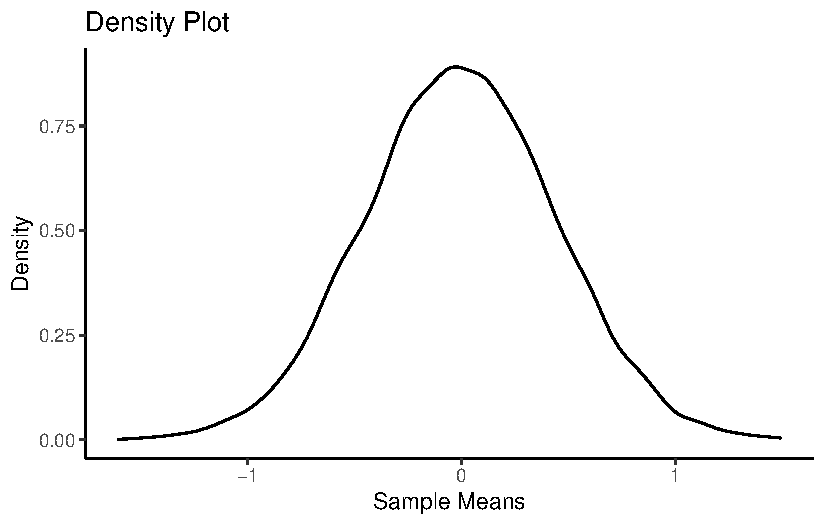
\includegraphics{./visualizing-data_files/figure-pdf/unnamed-chunk-1-1.pdf}

}

\end{figure}

\hypertarget{density-ridges}{%
\subsection{Density Ridges}\label{density-ridges}}

Using the \texttt{ggridges} package you can compare and see
distributions together.
\href{https://rdocumentation.org/packages/ggridges/versions/0.5.3}{Click
here} for the package documentation.

\begin{Shaded}
\begin{Highlighting}[]
\CommentTok{\# create density ridges with 3 randomly sampled distributions }
\NormalTok{samples\_df }\SpecialCharTok{\%\textgreater{}\%}
  \FunctionTok{ggplot}\NormalTok{(}\FunctionTok{aes}\NormalTok{(}\AttributeTok{x =}\NormalTok{ sample\_means, }\AttributeTok{y =}\NormalTok{ sample\_n, }\AttributeTok{fill =}\NormalTok{ sample\_n)) }\SpecialCharTok{+}
  \FunctionTok{geom\_density\_ridges}\NormalTok{(}\AttributeTok{alpha =}\NormalTok{ .}\DecValTok{7}\NormalTok{) }\SpecialCharTok{+} 
  \FunctionTok{labs}\NormalTok{(}\AttributeTok{title =} \StringTok{"Density Ridges Plot"}\NormalTok{, }\AttributeTok{x =}\StringTok{"Sample Means"}\NormalTok{, }\AttributeTok{y =} \StringTok{"Sample ID"}\NormalTok{) }\SpecialCharTok{+}
  \FunctionTok{theme\_classic}\NormalTok{()}
\end{Highlighting}
\end{Shaded}

\begin{verbatim}
Picking joint bandwidth of 0.0467
\end{verbatim}

\begin{figure}[H]

{\centering 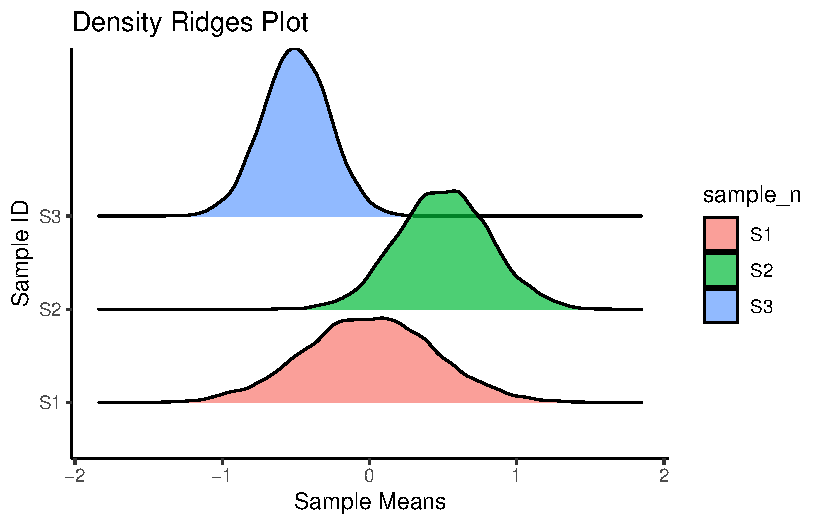
\includegraphics{./visualizing-data_files/figure-pdf/unnamed-chunk-3-1.pdf}

}

\end{figure}

\hypertarget{histogram}{%
\subsection{Histogram}\label{histogram}}

Using a histogram is another common way to show a distribution. It may
look like a ``bar char'' with many bars, however each ``bar'' is a bin,
and it represents a range of numbers that falls within it's respective
bin. The height of the ``bar'' shows a count of how many values fall
within a bin.

\begin{Shaded}
\begin{Highlighting}[]
\CommentTok{\# create histogram with random data }
\NormalTok{sample\_means\_df }\SpecialCharTok{\%\textgreater{}\%}
  \FunctionTok{ggplot}\NormalTok{(}\FunctionTok{aes}\NormalTok{(}\AttributeTok{x =}\NormalTok{ sample\_means)) }\SpecialCharTok{+}
  \FunctionTok{geom\_histogram}\NormalTok{(}\AttributeTok{bins =} \DecValTok{30}\NormalTok{) }\SpecialCharTok{+}
  \FunctionTok{labs}\NormalTok{(}\AttributeTok{title =} \StringTok{"Histogram"}\NormalTok{, }\AttributeTok{y =} \StringTok{"Count"}\NormalTok{, }\AttributeTok{x =} \StringTok{"Sample Means"}\NormalTok{) }\SpecialCharTok{+}
  \FunctionTok{theme\_classic}\NormalTok{()}
\end{Highlighting}
\end{Shaded}

\begin{figure}[H]

{\centering 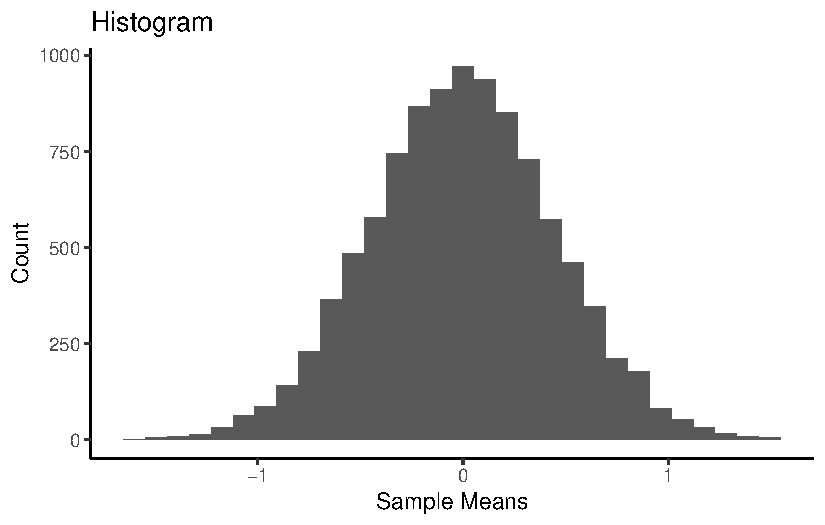
\includegraphics{./visualizing-data_files/figure-pdf/unnamed-chunk-4-1.pdf}

}

\end{figure}

\hypertarget{boxplot}{%
\subsection{Boxplot}\label{boxplot}}

Boxplots can be a useful way to show a distribution, but the
distribution is hidden behind each box meaning it could be
misinterpreted.

\begin{Shaded}
\begin{Highlighting}[]
\CommentTok{\# create boxplots with random data}
\NormalTok{samples\_df }\SpecialCharTok{\%\textgreater{}\%}
  \FunctionTok{ggplot}\NormalTok{(}\FunctionTok{aes}\NormalTok{(}\AttributeTok{x =}\NormalTok{ sample\_n, }\AttributeTok{y =}\NormalTok{ sample\_means, }\AttributeTok{fill =}\NormalTok{ sample\_n)) }\SpecialCharTok{+}
  \FunctionTok{geom\_boxplot}\NormalTok{() }\SpecialCharTok{+}
  \FunctionTok{labs}\NormalTok{(}\AttributeTok{title =} \StringTok{"Boxplot"}\NormalTok{) }\SpecialCharTok{+}
  \FunctionTok{theme\_classic}\NormalTok{()}
\end{Highlighting}
\end{Shaded}

\begin{figure}[H]

{\centering 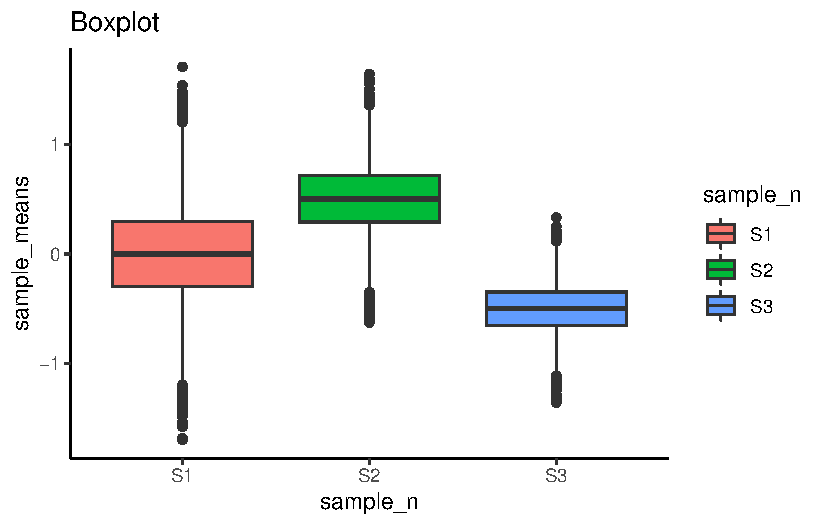
\includegraphics{./visualizing-data_files/figure-pdf/unnamed-chunk-5-1.pdf}

}

\end{figure}

\hypertarget{violin-chart}{%
\subsection{Violin Chart}\label{violin-chart}}

Similar to a boxplot but shows the shape of a distribution better.

\begin{Shaded}
\begin{Highlighting}[]
\CommentTok{\# create violin charts with random data}
\NormalTok{samples\_df }\SpecialCharTok{\%\textgreater{}\%}
  \FunctionTok{ggplot}\NormalTok{(}\FunctionTok{aes}\NormalTok{(}\AttributeTok{x =}\NormalTok{ sample\_n, }\AttributeTok{y =}\NormalTok{ sample\_means, }\AttributeTok{fill =}\NormalTok{ sample\_n)) }\SpecialCharTok{+}
  \FunctionTok{geom\_violin}\NormalTok{() }\SpecialCharTok{+}
  \FunctionTok{labs}\NormalTok{(}\AttributeTok{title =} \StringTok{"Violin Chart"}\NormalTok{) }\SpecialCharTok{+}
  \FunctionTok{theme\_classic}\NormalTok{()}
\end{Highlighting}
\end{Shaded}

\begin{figure}[H]

{\centering 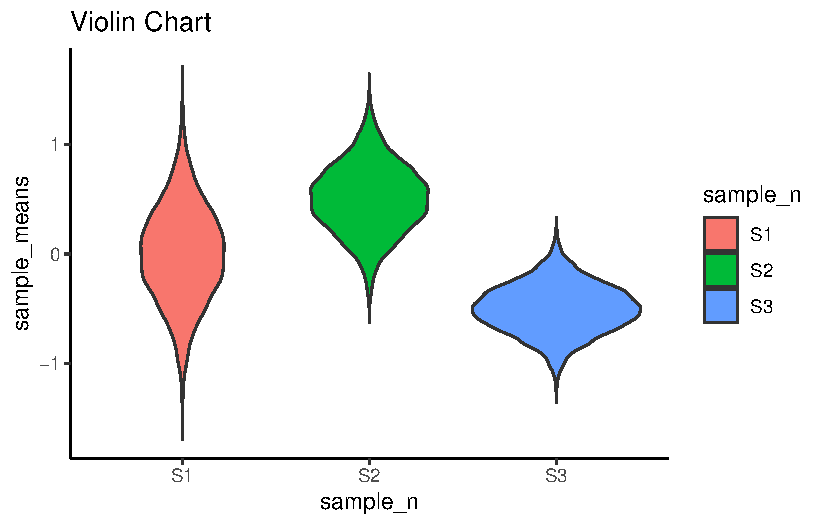
\includegraphics{./visualizing-data_files/figure-pdf/unnamed-chunk-6-1.pdf}

}

\end{figure}

\hypertarget{comparisons}{%
\section{Comparisons}\label{comparisons}}

For this group the visuals compare insights for the audience.

\hypertarget{bar-chart}{%
\subsection{Bar Chart}\label{bar-chart}}

Bar charts are very simple and effective at conveying information, never
underestimate the power of a bar chart.

\begin{Shaded}
\begin{Highlighting}[]
\CommentTok{\# read in iris dataset }
\NormalTok{iris\_df }\OtherTok{\textless{}{-}}\NormalTok{ iris }\SpecialCharTok{\%\textgreater{}\%}
  \FunctionTok{clean\_names}\NormalTok{()}

\CommentTok{\# group the data by species, then summarize the avg petal width for each species}
\NormalTok{iris\_df }\SpecialCharTok{\%\textgreater{}\%} 
  \FunctionTok{group\_by}\NormalTok{(species) }\SpecialCharTok{\%\textgreater{}\%}
  \FunctionTok{summarize}\NormalTok{(}\AttributeTok{avg\_petal\_width =} \FunctionTok{mean}\NormalTok{(petal\_width)) }\SpecialCharTok{\%\textgreater{}\%}
  \FunctionTok{ggplot}\NormalTok{(}\FunctionTok{aes}\NormalTok{(}\AttributeTok{x =}\NormalTok{ species, }\AttributeTok{y =}\NormalTok{ avg\_petal\_width, }\AttributeTok{fill =}\NormalTok{ species)) }\SpecialCharTok{+}
  \FunctionTok{geom\_col}\NormalTok{() }\SpecialCharTok{+}
  \FunctionTok{labs}\NormalTok{(}\AttributeTok{title =} \StringTok{"Bar Chart"}\NormalTok{, }\AttributeTok{y =} \StringTok{"Avg Petal Width"}\NormalTok{, }\AttributeTok{x =} \StringTok{"Species"}\NormalTok{) }\SpecialCharTok{+}
  \FunctionTok{theme\_classic}\NormalTok{()}
\end{Highlighting}
\end{Shaded}

\begin{figure}[H]

{\centering 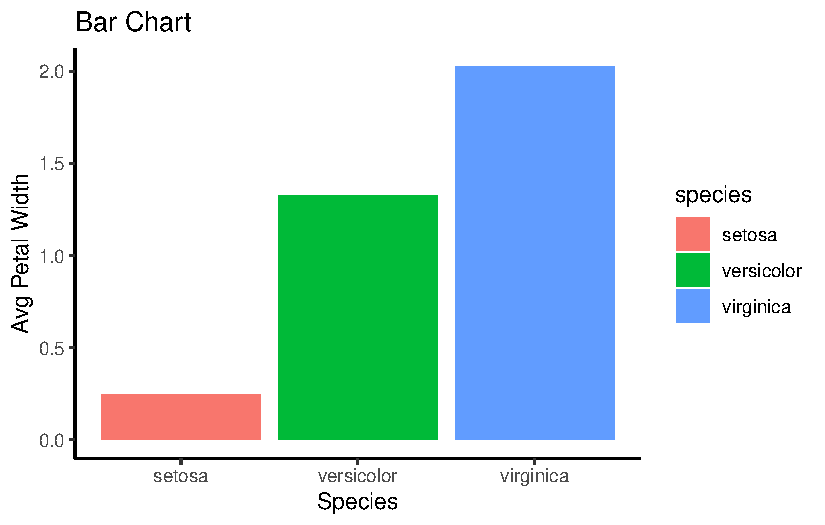
\includegraphics{./visualizing-data_files/figure-pdf/unnamed-chunk-8-1.pdf}

}

\end{figure}

\hypertarget{horizontal-bar-chart}{%
\subsection{Horizontal Bar Chart}\label{horizontal-bar-chart}}

Similar to a bar chart, but a horizontal version, can be useful but when
viewing, stakeholders can more easily distinguish a difference in the
vertical counterpart than in the horizontal bar chart. This is the same
bar chart as above, created with \texttt{+\ geom\_col()} but to rotate
the plot I used the \texttt{+\ coord\_flip()} function.

\begin{Shaded}
\begin{Highlighting}[]
\CommentTok{\# create horizontal bar chart}
\NormalTok{iris\_df }\SpecialCharTok{\%\textgreater{}\%} 
  \FunctionTok{group\_by}\NormalTok{(species) }\SpecialCharTok{\%\textgreater{}\%}
  \FunctionTok{summarize}\NormalTok{(}\AttributeTok{avg\_petal\_width =} \FunctionTok{mean}\NormalTok{(petal\_width)) }\SpecialCharTok{\%\textgreater{}\%}
  \FunctionTok{ggplot}\NormalTok{(}\FunctionTok{aes}\NormalTok{(}\AttributeTok{x =}\NormalTok{ species, }\AttributeTok{y =}\NormalTok{ avg\_petal\_width, }\AttributeTok{fill =}\NormalTok{ species)) }\SpecialCharTok{+}
  \FunctionTok{geom\_col}\NormalTok{() }\SpecialCharTok{+}
  \FunctionTok{labs}\NormalTok{(}\AttributeTok{title =} \StringTok{"Horizontal Bar Chart"}\NormalTok{, }\AttributeTok{y =} \StringTok{"Avg Petal Width"}\NormalTok{, }\AttributeTok{x =} \StringTok{"Species"}\NormalTok{) }\SpecialCharTok{+}
  \FunctionTok{theme\_classic}\NormalTok{() }\SpecialCharTok{+}
  \FunctionTok{coord\_flip}\NormalTok{()}
\end{Highlighting}
\end{Shaded}

\begin{figure}[H]

{\centering 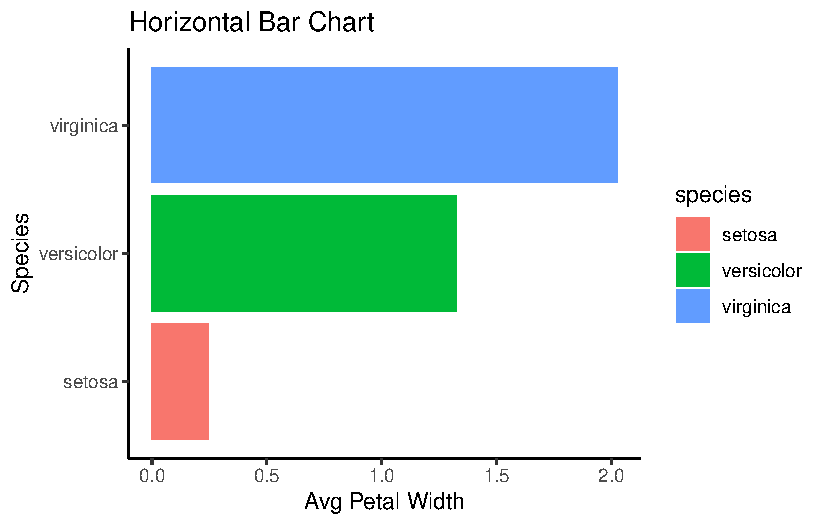
\includegraphics{./visualizing-data_files/figure-pdf/unnamed-chunk-9-1.pdf}

}

\end{figure}

\hypertarget{line-chart}{%
\subsection{Line Chart}\label{line-chart}}

Line charts are essential when working time.

\begin{Shaded}
\begin{Highlighting}[]
\CommentTok{\# read in chickweight dataset}
\NormalTok{chick\_df }\OtherTok{\textless{}{-}}\NormalTok{ ChickWeight }\SpecialCharTok{\%\textgreater{}\%}
  \FunctionTok{clean\_names}\NormalTok{()}

\CommentTok{\# filter and group by chick 1, 21, 45}
\NormalTok{chick\_df }\SpecialCharTok{\%\textgreater{}\%}
  \FunctionTok{filter}\NormalTok{(chick }\SpecialCharTok{==} \DecValTok{1}\SpecialCharTok{|}\NormalTok{chick }\SpecialCharTok{==} \DecValTok{21}\SpecialCharTok{|}\NormalTok{chick }\SpecialCharTok{==} \DecValTok{45}\NormalTok{) }\SpecialCharTok{\%\textgreater{}\%}
  \FunctionTok{group\_by}\NormalTok{(chick) }\SpecialCharTok{\%\textgreater{}\%}
  \FunctionTok{ggplot}\NormalTok{(}\FunctionTok{aes}\NormalTok{(}\AttributeTok{x =}\NormalTok{ time, }\AttributeTok{y =}\NormalTok{ weight, }\AttributeTok{color =}\NormalTok{ diet)) }\SpecialCharTok{+} 
  \FunctionTok{geom\_line}\NormalTok{(}\AttributeTok{size =}\NormalTok{ .}\DecValTok{8}\NormalTok{) }\SpecialCharTok{+}
  \FunctionTok{labs}\NormalTok{(}\AttributeTok{title =} \StringTok{"Line Chart"}\NormalTok{, }\AttributeTok{x =} \StringTok{"Time"}\NormalTok{, }\AttributeTok{y =} \StringTok{"Chicken Weight"}\NormalTok{) }\SpecialCharTok{+}
  \FunctionTok{theme\_classic}\NormalTok{()}
\end{Highlighting}
\end{Shaded}

\begin{figure}[H]

{\centering 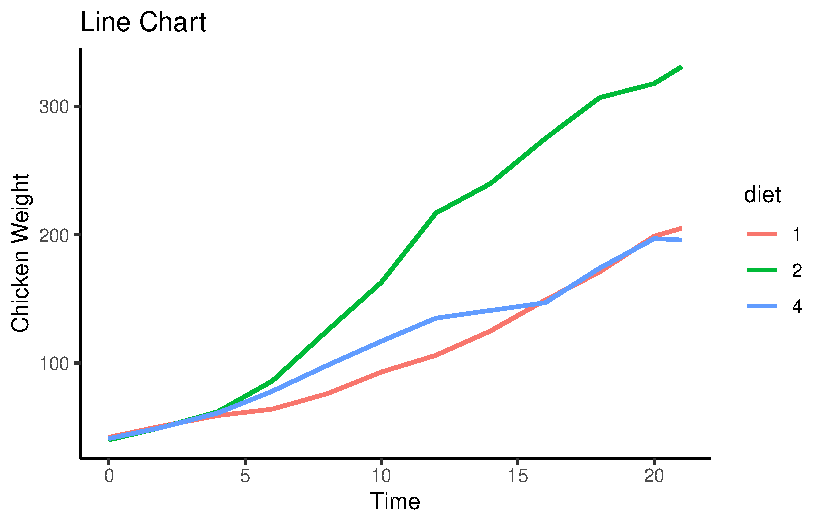
\includegraphics{./visualizing-data_files/figure-pdf/unnamed-chunk-10-1.pdf}

}

\end{figure}



\end{document}
